\documentclass[tikz,border=5pt]{standalone}
\usepackage[UTF8]{ctex}
\usepackage{amsmath,amssymb}
\usetikzlibrary{arrows.meta,calc,angles,quotes,decorations.pathmorphing}
\definecolor{ink}{HTML}{243447}\definecolor{blue}{HTML}{2765A2}
\definecolor{green}{HTML}{3F7D5B}\definecolor{red}{HTML}{B74739}
\tikzset{body/.style={draw=ink,thick},vec/.style={draw=blue,thick,-{Latex}},guide/.style={gray!65,dashed},dim/.style={ink,{Latex}-{Latex}},line cap=round,line join=round}
\begin{document}
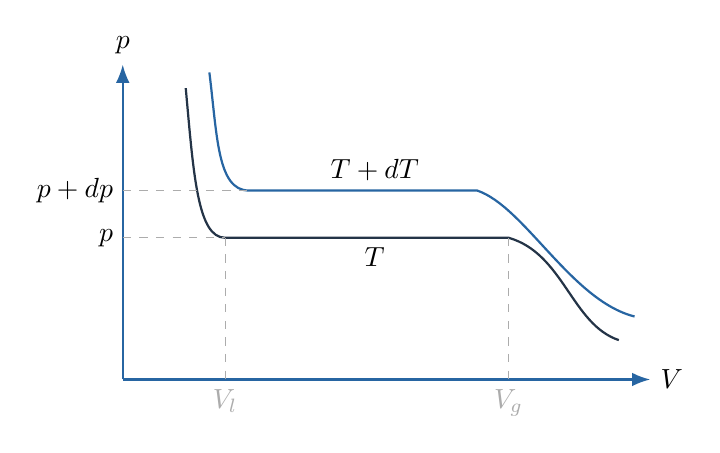
\begin{tikzpicture}
\draw[vec](0,0)--(6.7,0)node[right]{$V$};
\draw[vec](0,0)--(0,4)node[above]{$p$};
\draw[ink,thick](.8,3.7)..controls(.9,2.6)and(.95,1.8)..(1.3,1.8)--(4.9,1.8)..controls(5.6,1.6)and(5.7,.7)..(6.3,.5);
\draw[blue,thick](1.1,3.9)..controls(1.2,3.1)and(1.2,2.4)..(1.6,2.4)--(4.5,2.4)..controls(5.1,2.2)and(5.7,1)..(6.5,.8);
\draw[guide](0,1.8)--(1.3,1.8); \draw[guide](0,2.4)--(1.6,2.4);
\node[left]at(0,1.8){$p$};\node[left]at(0,2.4){$p+dp$};
\node[above]at(3.2,2.4){$T+dT$};\node[below]at(3.2,1.8){$T$};
\draw[guide](1.3,1.8)--(1.3,0)node[below]{$V_l$};
\draw[guide](4.9,1.8)--(4.9,0)node[below]{$V_g$};
\end{tikzpicture}
\begin{tikzpicture}
\draw[vec](0,0)--(7,0)node[right]{$V$};
\draw[vec](0,0)--(0,3.8)node[above]{$p$};
\fill[blue!12](1.3,2.4)--(5.3,2.4)--(5.45,1.6)--(1.45,1.6)--cycle;
\draw[vec](1.3,2.4)--(5.3,2.4)node[midway,above]{吸热：$Q_h\simeq\lambda_{\rm mol}$};
\draw[vec](5.45,1.6)--(1.45,1.6)node[midway,below]{放热：凝结};
\draw[green,thick,-{Latex}](5.3,2.4)..controls(5.38,2.1)and(5.4,1.9)..(5.45,1.6);
\draw[green,thick,-{Latex}](1.45,1.6)..controls(1.4,1.9)and(1.38,2.1)..(1.3,2.4);
\node[green,right]at(5.6,2){绝热连接};
\draw[dim](.8,1.6)--(.8,2.4)node[midway,left]{$dp$};
\draw[dim](1.45,.5)--(5.45,.5)node[midway,below]{$V_g-V_l$};
\node at(3.4,2){$W\simeq dp(V_g-V_l)$};
\node at(3.5,-.8){仅表示一阶面积；端点移动产生二阶修正};
\end{tikzpicture}
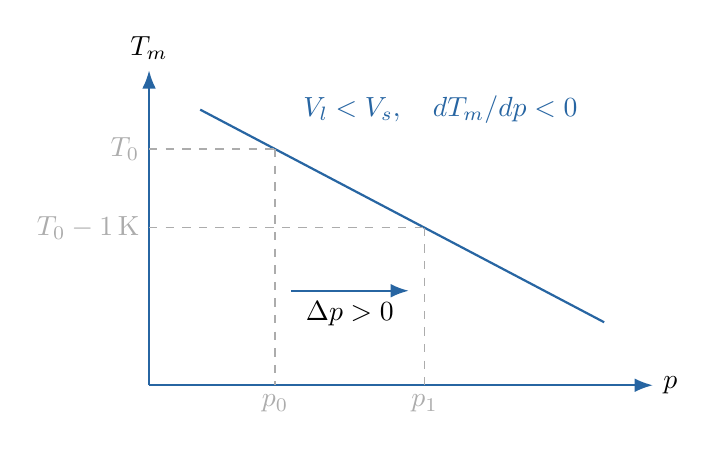
\begin{tikzpicture}
\draw[vec](0,0)--(6.4,0)node[right]{$p$};
\draw[vec](0,0)--(0,4)node[above]{$T_m$};
\draw[blue,thick](.65,3.5)--(5.78,.8);
\draw[guide](1.6,3)--(1.6,0)node[below]{$p_0$};\draw[guide](3.5,2)--(3.5,0)node[below]{$p_1$};
\draw[guide](0,3)--(1.6,3)node[left,pos=0]{$T_0$};
\draw[guide](0,2)--(3.5,2)node[left,pos=0]{$T_0-1\,\mathrm K$};
\draw[vec](1.8,1.2)--(3.3,1.2)node[midway,below]{$\Delta p>0$};
\node[blue]at(3.7,3.5){$V_l<V_s,\quad dT_m/dp<0$};
\end{tikzpicture}
\end{document}
